\section{Použití trezoru}
Mechanické verze trezoru M1 a M2 měly na akcích a v kroužcích děti možnost jen stavět. První akce založená na trezoru, která neobsahovala jen stavbu, využívala až variantu M3.

Protože na akci byly menší děti, byl trezor místo klasické číselné stupnice  vybaven obrázkovým kódem, jak je vidět na obrázku \ref{fig:M3-trpaslici}.

\begin{figure}[htbp]
    \centering
    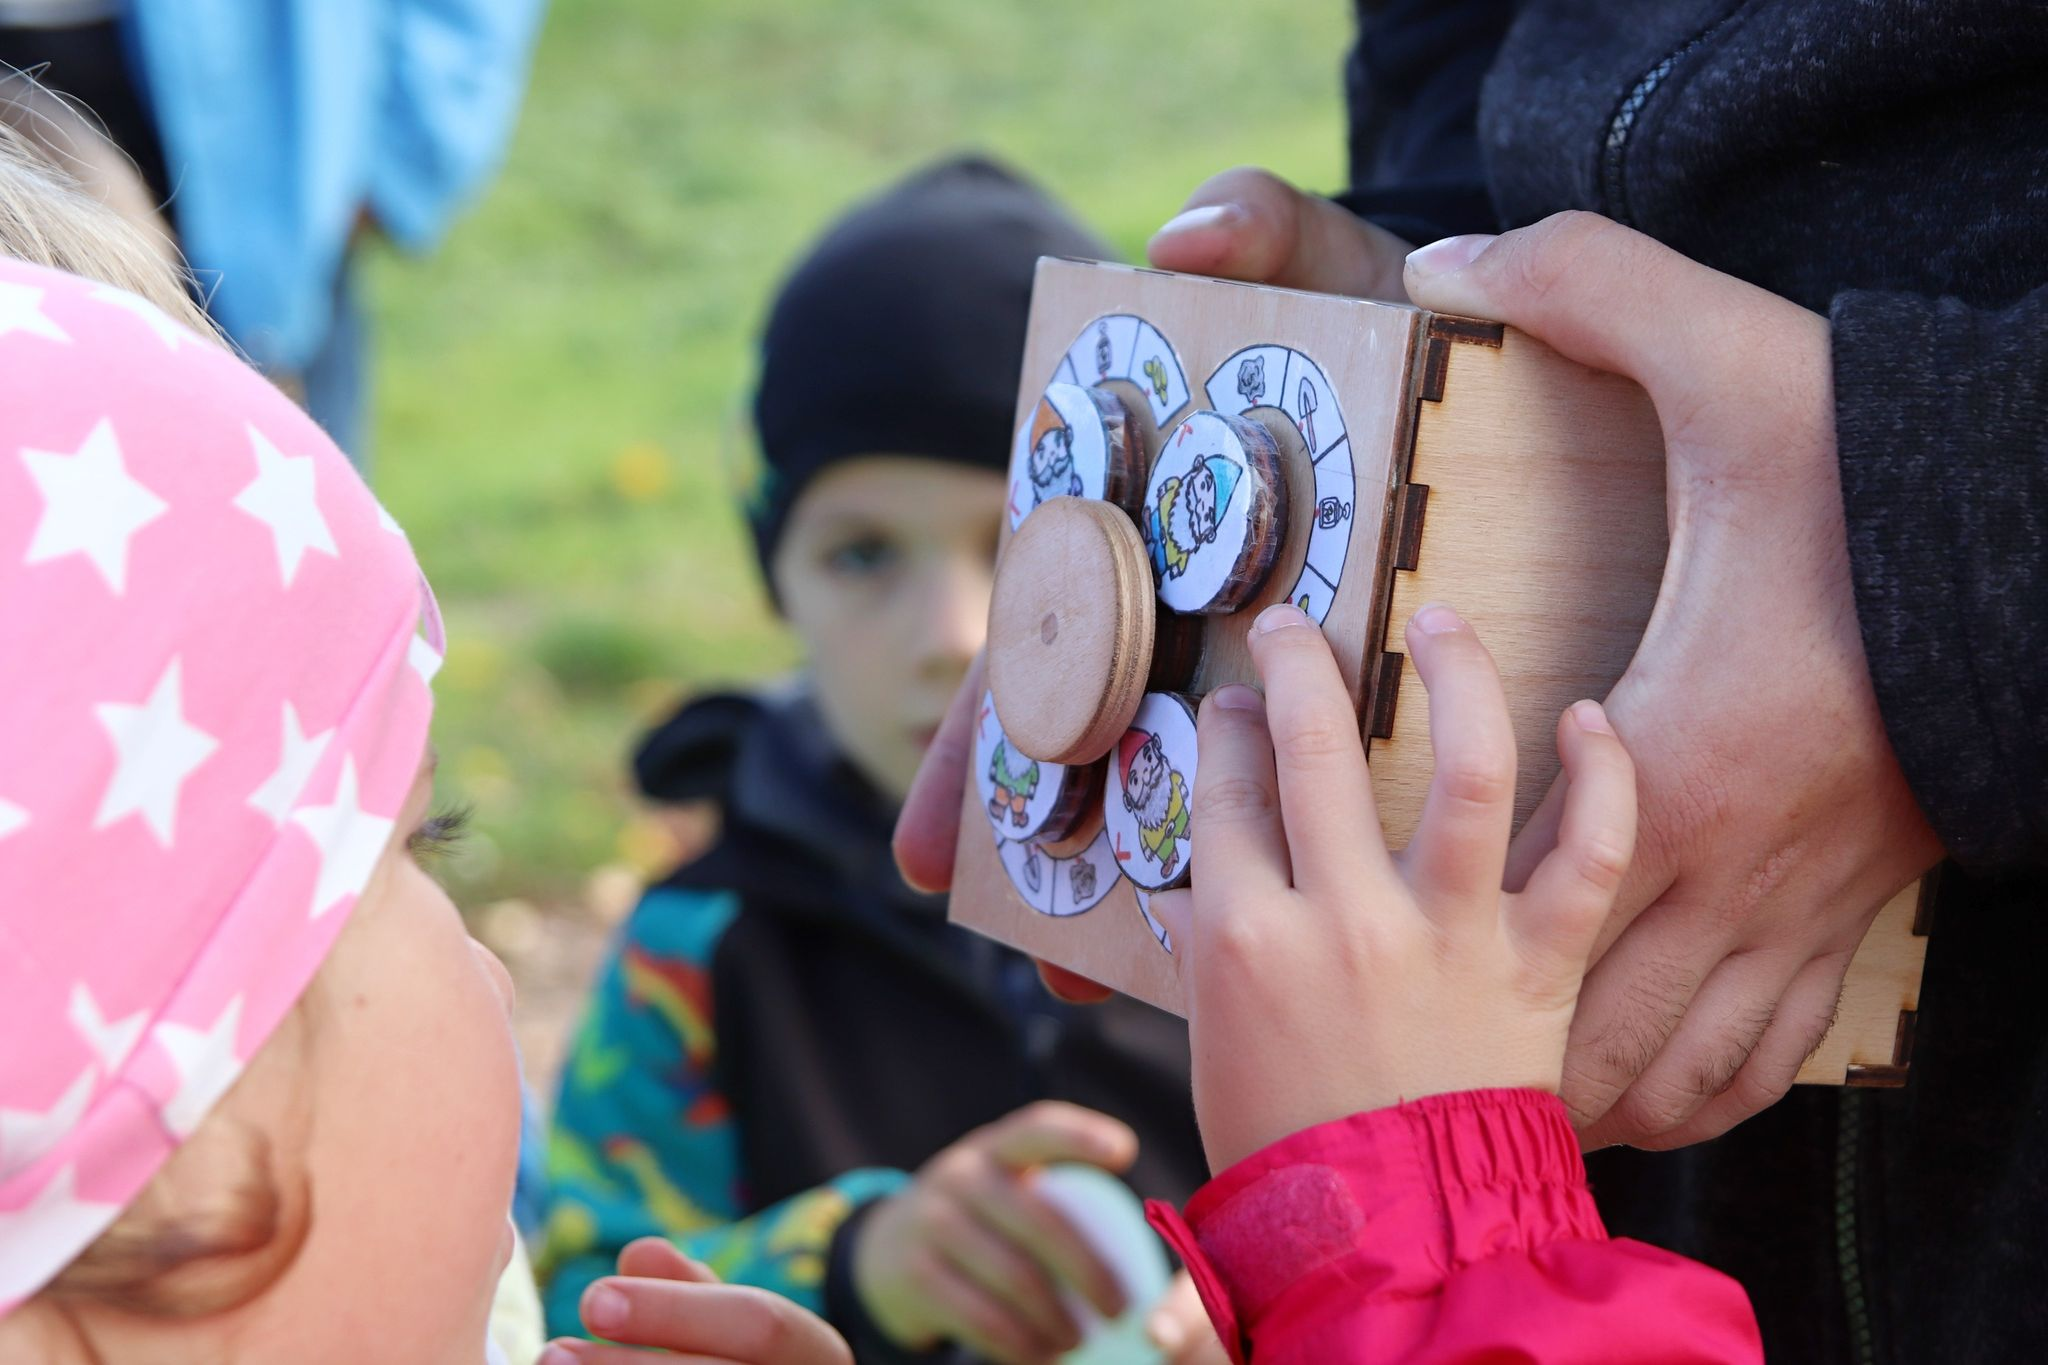
\includegraphics[width=\textwidth]{kapitoly/obrazky/M3/trpaslici.png}
    \caption{Render varianty M3}
    \label{fig:M3-trpaslici}
\end{figure}
